\documentclass[aspectratio=169]{beamer}
\usetheme{A}

\usepackage{stmaryrd}
\usepackage{fontspec}
\usepackage{unicode-math}
\setmainfont{Libertinus Serif}
\setsansfont{Libertinus Sans}
\setmonofont{Libertinus Mono}
\setmathfont{Libertinus Math}

\usepackage{xcolor}
\usepackage{tabularx}
\usepackage{booktabs}
\usepackage{proof}
\usepackage{eqparbox}

\usepackage[normalem]{ulem}

\definecolor{light}{rgb}{0.38,0.38,0.38}
\newcommand{\light}[1]{\textcolor{light}{#1}}

\usepackage{tikz}
\usetikzlibrary{decorations.pathreplacing}
\usepackage{relsize}
\usepackage{enumitem}
\setlist[itemize]{label=\textcolor{pred}{$\bullet$}, topsep=0pt, itemsep=0pt}
\setlist[itemize,2]{label=\textcolor{pred}{$\circ$}, topsep=0pt, itemsep=0pt,leftmargin=1.5em}

%
\newcommand{\rulestyle}[1]{#1}
\newcommand{\Ax}{\rulestyle{Ax}}
\newcommand{\EX}{\rulestyle{Ex}}
\newcommand{\li}{\to}
\newcommand{\bs}{\backslash}
\newcommand{\ty}[1]{#1}
\newcommand{\te}[1]{#1}
\newcommand{\appr}{\triangleright}
\newcommand{\appl}{\triangleleft}
\newcommand{\lambdar}{\lambda^r}
\newcommand{\lambdal}{\lambda^l}
\renewcommand{\otimes}{⊗}
\newcommand{\crossmark}{✘}
\newcolumntype{C}{>{\centering\arraybackslash}X}
\newcommand{\alertat}[2]{\alt<#1>{\alert{#2}}{#2}}
\newcommand{\lightat}[2]{\alt<#1>{\light{#2}}{#2}}
\newcommand{\showat}[2]{\alt<#1>{#2}{}}
\newcommand{\strat}[2]{\alt<#1>{\sout{#2}}{#2}}
\newcommand{\caseof}[3]{\text{case }{\te{#1}}\text{ of }{\te{#2}}\text{ in }{\te{#3}}}
\renewcommand{\emptyset}{()}
\newcommand{\inferat}[4][]{%
	\alt<#2>{
		\infer[#1]{#3}{#4}
	}{%
		\deduce[\visible<#2>{#1}]{\visible<#2>{#3}}{#4}
	}%
}
\newcommand{\infereat}[4][]{%
	\alt<#2>{
		\infer=[#1]{#3}{#4}
	}{%
		\deduce[\visible<#2>{#1}]{\visible<#2>{#3}}{#4\vspace{2pt}}
	}%
}
\newcommand{\subst}[1]{\llbracket{#1}\rrbracket}
\renewcommand{\alert}[1]{\textcolor{pred}{#1}}
\newcommand{\Lex}{\rulestyle{Lex}}
\newcommand{\w}[1]{\text{#1}}
\newcommand{\sbr}{\mathbin{\cdot}}
\newcommand{\Ass}{\rulestyle{A}}

\title{Grammaticality as Provability}
\date{%
	\\
	Groningen Logic Seminar\\
	May 2025
	\vspace{6em}
}
\author{\light{Konstantinos Kogkalidis}}
\renewcommand{\arraystretch}{1.15}


\begin{document}

\maketitle

\begin{frame}{The Big Picture}
	\smaller
	
	\begin{minipage}[t]{0.45\textwidth}
	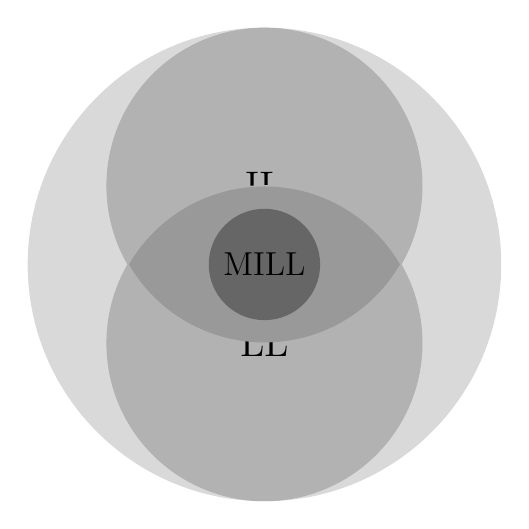
\begin{tikzpicture}[
		one/.style={fill=gray!30, draw=gray!30},
		two/.style={fill=gray!60, draw=gray!60},
		three/.style={fill=gray!80, draw=gray!80},
		four/.style={fill=black!60, draw=black!60}
		]
		\draw[one] (0,0) circle (3);
		\visible<1>{\node at (0, 0) {\Large CL};}
		\visible<2,4->{
		\draw[two] (0, 1) circle (2);
		\visible<2>{\node at (0, 1) {\Large IL};}
		}
		\visible<3,4->{
		\draw[two] (0, -1) circle (2);
		\visible<3>{\node at (0, -1) {\Large LL};}
		}
		\visible<4->{
		\clip (0, 1) circle (1.99);
		\clip (0, -1) circle (1.99);
		\draw[three] (0,0) circle (2.6);
		\visible<4>{\node at (0, 0) {\Large ILL};}
		}
		\visible<5->{
		\draw[four] (0,0) circle (0.7);
		\visible<5>{\node at (0, 0) {\large MILL};}
		}
	\end{tikzpicture}%
	\end{minipage}\hfill%
	\begin{minipage}[t]{0.55\textwidth}
	\vspace{-5cm}
	\begin{itemize}
		\item \eqmakebox[logic][l]{\alert{CL}} \light{(folklore\dots)}
		\visible<2->{
		\item \eqmakebox[logic][l]{\alert{IL}} \light{(Heyting, 1930)}\\
		{no excluded middle, no involutive negation}
		}
		\visible<3->{
		\item \eqmakebox[logic][l]{\alert{LL}} \light{(Girard, 1987)}\\
		{truth $\equiv$ resource; no weakening, no contraction}
		}
		\visible<4->{
		\item \eqmakebox[logic][l]{\alert{ILL}} \\
		{= LL $\cap$ IL}
		}
		\visible<5->{
		\item \eqmakebox[logic][l]{\alert{MILL}} \\
		{= ILL without additives}
		}
	\end{itemize}\vfill
	\end{minipage}
\end{frame}

\begin{frame}{MILL\\
\smaller\light{\quad\alt<10->{term calculus}{typing rules}}}
	\smaller
	
	\begin{minipage}{.5\textwidth}
		\begin{tabular}{@{}r@{ }l@{}}
		 	\multicolumn{2}{@{}l}{\textbf{Types}}\\
			$\ty{A, B, C}$ & $:= p \ | \ \ty{A\li B} \ | \ \ty{A\otimes B}$ \qquad \light{($p \in Prim.$)}\\
		    \addlinespace
			\multicolumn{2}{@{}l}{\uncover<2->{\textbf{Structures}}}\\
		  	\uncover<2->{
		   	$\Gamma, \Delta$ & $:= \ \emptyset \ | \ \Gamma\sbr \ty{A}$
		   	}
		\end{tabular}
	\end{minipage}
	\vspace{1em}
	
	\centering
	\begin{tabularx}{0.8\textwidth}{@{}CC@{}}
	\multicolumn{2}{@{}c@{}}{\uncover<3,9->{\alertat{3}{
		$\infer[\Ax]{\showat{10-}{\light{\te{x}} : }\ty{A} \vdash \showat{10-}{\light{\te{x}} : }\ty{A}}{}$}}}\\
	\addlinespace
	\uncover<4,9->{%
	\alertat{4}{
	$\infer[\li_E]{\Gamma\sbr \Delta \vdash \showat{10-}{\light{\te{s~t}} : }\ty{B}}{\Gamma \vdash \showat{10-}{\light{\te{s}} : }\ty{A \li B} & \Delta \vdash \showat{10-}{\light{\te{t}} : }\ty{A}}$
	}}
	&
	\uncover<5,9->{%
	\alertat{5}{
	$\infer[\li_I]{\Gamma \vdash \showat{10-}{\light{\te{\lambda x.s}} : }\ty{A \li B}}{\Gamma\sbr \showat{10}{\light{\te{x}} : }A \vdash \showat{10}{\light{\te{s}} : }B}$
	}}\\
	\addlinespace
	\uncover<7,9->{\alertat{7}{$\infer[\otimes_E]{\Gamma\sbr \Delta \vdash \showat{10-}{\light{\caseof{s}{(x, y)}{t}} : }C}{\Gamma \vdash \showat{10-}{\light{\te{s}} : }\ty{A\otimes B} & \Delta\sbr\showat{10-}{\light{\te{x}} : }\ty{A}\sbr \showat{10-}{\light{\te{y}} : }\ty{B} \vdash \showat{10-}{\light{\te{t}} : }\ty{C}}$}}
	&
	\uncover<6,9->{
	\alertat{6}{
	$\infer[\otimes_I]{\Gamma\sbr \Delta \vdash \showat{10-}{\light{\te{(x, y)}} : }\ty{A \otimes B}}{\Gamma \vdash \showat{10-}{\light{\te{x}} : }\ty{A} & \Delta \vdash \showat{10-}{\light{\te{y}} : }\ty{B}}$}}\\
	\addlinespace
	\multicolumn{2}{@{}c@{}}{
	\uncover<8->{
	\alertat{8}{
	$\infer=[\EX]{\Gamma\sbr \ty{B}\sbr \ty{A}\sbr \Delta \vdash \ty{C}}{\Gamma\sbr \ty{A}\sbr \ty{B}\sbr \Delta \vdash \ty{C}}$
	}}}
	\end{tabularx}
\end{frame}

\begin{frame}{Invertible Inferences}
	\smaller
	\begin{minipage}{.5\textwidth}
	\[
	\infereat{4-}{
			\ty{A_1 \otimes \dots \otimes A_n} \vdash \ty{B} 
		}{
			\infereat{3-}{
				 	\emptyset \vdash \ty{(A_1 \otimes \dots \otimes A_n)\li B}
		}{
					\infereat{2-}{
							\emptyset \vdash \ty{A_1\li \dots \li A_n\li B}
						}{
							 \Gamma_{\light{[\ty{A_1}\sbr ~\dots~ \sbr \ty{A_n}]}} \vdash \ty{B}
						}
				}
		}
	\]
	\vspace{0.5em}
	\visible<5->{
	\uncover<-6>{
	\[
		\infer=[\Gamma' \in \mathsf{S}_n(\Gamma)]{\Gamma'~ \vdash \ty{B}}{\Gamma \vdash \ty{B}}
	\]}}
	\end{minipage}
	
	\visible<6->{	
	\begin{tikzpicture}[overlay,remember picture,xshift=18em,yshift=6.5em]
	   	\draw [decoration={brace,amplitude=5pt,mirror,raise=2pt},decorate,thick,draw=pred]
    (0, -1.6) -- (0, 1.6) node[midway,right=1pt,align=left] {
    	\begin{minipage}{24em}
    	\begin{itemize}
    		\item premises are \strat{7-}{\lightat{7-}{\alertat{-6}{\textit{multisets}}}} \visible<7->{\alert{\textit{sequences}} ($n!$ as many)}
    		\item \alert{$\otimes$} and \alert{$\sbr$} are \textit{\alert{variadic}} \strat{7-}{\lightat{7-}{and \textit{\alertat{-6}{order-insensitive}}}}
    		\item[] \vdots
	    \end{itemize}    	
    	\end{minipage}
	    };
	    \visible<7->{
	    	\node[pred, very thick, scale=5.5] at (-2.2, -1.2) {$\crossmark$};
	    }
	\end{tikzpicture}
	}
\end{frame}

\begin{frame}{Going Sub\textsuperscript{(2)}structural
\\
\quad\smaller\light{A world without exchange}}
	\smaller
	\alt<2->{
		\textbf{Now}: \\
		\qquad$
			\ty{A_1 \bs (A_2 \bs B)} \mathbin{\alert{\not\equiv}} \ty{A_2 \bs (A_1 \bs B)} \mathbin{\alert{\not\equiv}} \ty{(B / A_2) / A_1} \mathbin{\alert{\not\equiv}} \ty{(B / A_1) / A_2} \mathbin{\alert{\not\equiv}} \ty{(A_1 \bs B) / A_2} \mathbin{\alert{\not\equiv}} \ty{(A_2 \bs B) / A_1}
		$
		
		\hfill \light{all these just from $\ty{A_1\li A_2\li B}$ (!)} 
		\vfill
	
		\visible<3->{
		\textbf{Yet still}: \\
		\qquad$\ty{(A_1 \bs B)/A_2} \equiv \ty{A_1 \bs (B / A_2)}$
		
		\[
			\infer={
					\alert{\Gamma \vdash \ty{(A_1 \bs B) / A_2}}
				}{
					\infer={
						\Gamma\sbr \ty{A_2} \vdash \ty{A_1 \bs B}
					}{
						\infer={
							\ty{A_1}\sbr \Gamma\sbr \ty{A_2} \vdash \ty{B}
						}{
							\infer={
								\ty{A_1}\sbr \Gamma \vdash \ty{B / A_2}
							}{
								\alert{\Gamma \vdash \ty{A_1 \bs (B / A_2)}}
							}
						}
					}
				}
		\]
	}
	}{%
		Without \EX{}, $\li$ branches into two \alert{position-refined} variants: $\alert{/}$ and $\alert{\bs}$.\\ 
		~\light{Read: 
		\begin{tabular}{r@{ -- }l}
			$\ty{B / A}$ & ``$\ty{B}$ \textit{over} $\ty{A}$''\\
			$\ty{A \bs B}$ & ``$\ty{A}$ \textit{under} $\ty{B}$''
		\end{tabular}}\vspace{1em}
	
		\begin{center}\begin{tabularx}{0.8\textwidth}{@{}CC@{}}
		$
			\infer[\bs_E]{\Gamma\sbr \Delta \vdash \light{\te{s \appr t}} : \ty{B}}{\Gamma \vdash \light{\te{s}} : \ty{\alert{A}}  & \Delta \vdash \light{\te{t}} : \ty{\alert{A} \bs B}}
		$
		&
		$
			\infer[\bs_I]{\Gamma \vdash \light{\te{\lambdal x.s}} : \ty{\alert{A} \bs B}}{\light{\te{x}}: \ty{\alert{A}}, \Gamma \vdash \ty{B}}
		$\\
		\addlinespace\addlinespace\addlinespace
		$
			\infer[/_E]{\Gamma\sbr \Delta \vdash \light{\te{s\appl t}}:\ty{B}}{\Gamma \vdash \light{\te{s}}: \ty{B / \alert{A}}  & \Delta \vdash \light{\te{t}}: \ty{\alert{A}}}
		$
		&
		$
			\infer[/_I]{\Gamma \vdash \light{\te{\lambdar x.s}}: \ty{B / \alert{A}}}{\Gamma\sbr \light{\te{x}}: \ty{\alert{A}} \vdash \light{\te{s}}: \ty{B}}
		$
		\\
		\addlinespace\addlinespace\addlinespace
		\multicolumn{2}{c}{
		$\infer[\otimes_E]{\Gamma\sbr \alert{\Delta}\sbr \alert{\Theta} \vdash \light{\caseof{s}{(x, y)}{t}} : C}{\Gamma \vdash \light{\te{s}} : \ty{A\otimes B} & \alert{\Delta}\sbr \light{\te{x}} : \ty{A}, \light{\te{y}} : \ty{B}\sbr \alert{\Theta} \vdash \light{\te{t}} : \ty{C}}$
		}
		\end{tabularx}\end{center}
	}
\end{frame}

\begin{frame}{}
	\centering
	\vfil
	\light{The (invisible) culprit?}
\end{frame}

\begin{frame}{Going Sub\textsuperscript{(2)}structural
\\
\quad\smaller\light{A world without exchange or associativity}}
\smaller
	\begin{itemize}
		\item premises become \textit{\alert{trees}} ($C_{n-1}$ as many)
		\item \alert{$\otimes$} and \alert{$,$} become \textit{\alert{binary}}
		\item[] \vdots
	\end{itemize}\vspace{2em}

	\begin{center}\begin{tabularx}{0.8\textwidth}{@{}CC@{}}
	$
		\infer[\bs_E]{\alert{(}\Gamma\mathbin{\alert{\sbr}} \Delta\alert{)} \vdash \light{\te{s \appr t}} : \ty{B}}{\Gamma \vdash \light{\te{s}} : \ty{A}  & \Delta \vdash \light{\te{t}} : \ty{A \bs B}}
	$
	&
	$
		\infer[\bs_I]{\Gamma \vdash \light{\te{\lambdal x.s}} : \ty{A \bs B}}{\alert{(}\light{\te{x}}: \ty{A}\mathbin{\alert{\sbr}} \Gamma\alert{)} \vdash \ty{B}}
	$\\
	\addlinespace\addlinespace\addlinespace
	$
		\infer[/_E]{\alert{(}\Gamma\mathbin{\alert{\sbr}} \Delta\alert{)} \vdash \light{\te{s\appl t}}:\ty{B}}{\Gamma \vdash \light{\te{s}}: \ty{B / A}  & \Delta \vdash \light{\te{t}}: \ty{A}}
	$
	&
	$
		\infer[/_I]{\Gamma \vdash \light{\te{\lambdar x.s}}: \ty{B / A}}{\alert{(}\Gamma\mathbin{\alert{\sbr}} \light{\te{x}}: \ty{A}\alert{)} \vdash \light{\te{s}}: \ty{B}}
	$
	\\
	\addlinespace\addlinespace\addlinespace
	\multicolumn{2}{c}{
	$\infer[\otimes_E]{\Delta\subst{\alert{\Gamma}} \vdash \light{\caseof{s}{(x\sbr y)}{t}} : C}{\Gamma \vdash \light{\te{s}} : \ty{A\otimes B} & \Delta\subst{\alert{(}\light{\te{x}} : \ty{A}\mathbin{\alert{\sbr}} \light{\te{y}} : \ty{B}\alert{)}} \vdash \light{\te{t}} : \ty{C}}$
	}
	\end{tabularx}\end{center}
\end{frame}

\begin{frame}{The Small Picture\\
\quad\smaller\light{An alternative timeline}}
	\smaller
	
	\begin{minipage}[t]{0.45\textwidth}\centering\begin{tikzpicture}[
		g/.style={outer sep=6pt, inner sep=0pt,minimum width=4pt},e/.style={thick},
		scale=1.5
	]
		\node[g] (L) 	at (0,0)			{\alertat{1}{L}};
		\visible<2->{
		\node[g] (NL)	at (2, 0)			{\alertat{2}{NL}};
		\draw[e, ->] (L) -- (NL) node[midway,above]{-asso};
		}
		\visible<3->{
		\node[g] (LP)	at (0, -1.5)		{\alertat{3}{LP}};
		\draw[e, <-] (LP) -- (L) node[midway,left]{+comm};
		}
		\visible<4->{
		\node[g] (NLP)	at (2, -1.5)		{\alertat{4}{NLP}};
		\draw[e, ->] (NL) -- (NLP) node[midway,right]{+comm};
		\draw[e, ->] (NLP) -- (LP) node[midway,below]{+asso};
		}

	\end{tikzpicture}\end{minipage}\hfill
	\begin{minipage}[t]{0.55\textwidth}\vspace{-8em}\begin{itemize}
		\item \eqmakebox[logic][l]{\alert{L}} \light{(Lambek, 1958)}
		\visible<2->{
		\item \eqmakebox[logic][l]{\alert{NL}} \light{(Lambek, 1961)}
		}
		\visible<3->{
		\item \eqmakebox[logic][l]{\alert{LP}} \light{(van Benthem, 1983)}\\
		= MILL (!)
		}
		\visible<4->{
		\item \eqmakebox[logic][l]{\alert{NLP}} \light{(\textit{ditto})}
		}

	\end{itemize}\vfill\end{minipage}\vfill
	

	\visible<5->{
		\begin{center}
		\textbf{(N)L(P)}: Grammar Logics
		\end{center}\vfill
		
		\smaller
		\begin{flushright}
		\visible<6->{\light{
			\textit{%
				``Every mathematical discovery is made twice: once by a \strat{7-}{\lightat{7-}{logician}} \alt<7->{theoretical linguist}{} and once by a \strat{7-}{\lightat{7-}{computer scientist}} \alt<7->{logician}{}''\\
 -- P. Wadler \visible<7->{(retrofitted)}
 			}
		}}
		\end{flushright}
	}
\end{frame}

\begin{frame}{(N)L(P)\\
\quad\smaller\light{Executive Summary}
}\smaller\centering
	\begin{tabular}{@{}cccc@{}}
		Logic		& $\Gamma$	& Asso	& Comm\\
		\toprule
		LP			& multiset	& $✔$ 	& $✔$\\
		L			& string	& $✔$	& $\crossmark$\\
		NL			& tree		& $\crossmark$	& $\crossmark$\\
		NLP			& mobile	& $\crossmark$	& $✔$
	\end{tabular}

\end{frame}

\begin{frame}{Type-Logical Grammar 101\\
\smaller\quad\light{The idea}
}\smaller
	\begin{center}
	\begin{tabularx}{.8\textwidth}{@{}CCC@{}}
		\toprule
		\textbf{Language}			& \textbf{Logic}			& \textbf{Computation}\\
		\toprule
		grammar						& substructural logic 		& $\lambda$-calculus\\
		syntactic category			& formula					& type\\
		\alertat{2}{word}			& \alertat{2}{hypothesis}	& \alertat{2}{variable}\\
		phrasal composition 		& inference rule			& computation step\\
		grammaticality				& provability				& type inhabitation\\
		\multicolumn{3}{c}{\larger\vdots}\\
		sentence					& proof						& program\\
		parsing						& deduction					& computation
	\end{tabularx}\end{center}\vfill
	
	\visible<2->{
	\textbf{The lexicon} -- a mapping associating words and types\\
		\light{\quad $\Lex{} : \mathsf{Words}$ $\to$ $\mathcal{P}(\mathcal{U})$}
	}
\end{frame}


%\renewcommand{\Lex}{}
%\renewcommand{\Ax}{}

\begin{frame}{Type-Logical Grammar 102\\
\smaller\quad\light{Example derivation (L)}
}\smaller
	\[
		\infer[/_E]{(\w{the} \sbr (\w{violence} \sbr (\w{that} \sbr ((\w{the} \sbr \w{world}) \sbr \w{ignores})))) \vdash \ty{np}}{
			\infer[\Lex]{\ty{np / n}}{\w{the}}
			&
			\infer[\bs_E]{(\w{violence} \sbr (\w{that} \sbr ((\w{the} \sbr \w{world}) \sbr \w{ignores})))}{
				\hspace{1.5em}
				\infer[\Lex]{\ty{n}}{\w{violence}}
				&
				\hspace{1.5em}
				\infer[/_E]{(\w{that} \sbr ((\w{the} \sbr \w{world}) \sbr \w{ignores})) \vdash \ty{n\bs n}}{
					\infer[\Lex]{\ty{(n \bs n) / (s / np)}}{\w{that}} 
					&
					\infer[/_I]{((\w{the} \sbr \w{world}) \sbr \w{ignores}) \vdash \ty{s/np}}{
						\infer[\alert{\Ass}]{(\alert{(}(\w{the} \sbr \w{world}) \sbr \w{ignores}\alert{)} \sbr \ty{np}) \vdash \ty{s}}{
							\infer[\bs_E]{((\w{the} \cdot \w{world}) \cdot \alert{(}\w{ignores} \cdot \ty{np}\alert{)}) \vdash \ty{s}}{
								\infer[/_E]{(\w{the} \cdot \w{world}) \vdash \ty{np}}{
										\infer[\Lex]{\ty{np/n}}{\w{the}}
										&
										\infer[\Lex]{\ty{n}}{\w{world}}
								}
								&
								\infer[/_E]{(\w{ignores} \cdot \ty{np}) \vdash \ty{np \bs s}}{
									\infer[\Lex]{\ty{(np \bs s)/np}}{\w{ignores}}
									&
									\infer[\Ax]{\ty{np} \vdash np}{}
								}
							}
						}
					}
				}
			}
		}
	\]
\end{frame}

\end{document}